\documentclass{IEEEtran} 
\usepackage[utf8]{inputenc} %utf8 text character encoding
\usepackage[T1]{fontenc}
\usepackage{CJKutf8}
\usepackage{cite}
\usepackage{amsmath,amssymb,amsfonts,nccmath}
\usepackage{hyperref}
\hypersetup{colorlinks,linkcolor={blue},citecolor={blue},urlcolor={red}}  
\usepackage{cleveref} %Para usar crefrange
\usepackage{algorithm,algorithmic}
\usepackage{fancybox, graphicx}
\usepackage{textcomp}
\usepackage[font=footnotesize,labelfont=bf]{caption}
\usepackage[font=footnotesize,labelfont=bf]{subcaption}
\usepackage{graphicx}
\usepackage{color}
\usepackage{gensymb}
\usepackage{dblfloatfix}
\usepackage{lineno}
%\usepackage{biblatex}
\usepackage{enumitem}
\usepackage{wrapfig}
\usepackage{tikz}
\usepackage[autostyle]{csquotes}
\usepackage{listings}

\definecolor{backcolour}{rgb}{0.95,0.95,0.92}
\definecolor{codegreen}{rgb}{0,0.6,0}
\definecolor{codegray}{rgb}{0.5,0.5,0.5}
\definecolor{codepurple}{rgb}{0.58,0,0.82}



\newcommand{\squeezeup}{\vspace{-3mm}}
\usepackage{latexsym} 
\renewcommand{\arraystretch}{1.3}

\title{Practice 3: Signal Analysis: ASK simulation in Matlab}

\author{Alemón Pérez Alejandro, Álvarez Zamora Óscar Eduardo, Gallegos Ruiz Diana Abigail, Rojas Gómez Ian } 

\lstdefinestyle{mystyle}{
	backgroundcolor=\color{backcolour!19},   
	commentstyle=\color{codegreen},
	keywordstyle=\color{blue},
	numberstyle=\tiny\color{codegray},
	stringstyle=\color[rgb]{0.639,0.082,0.082}\ttfamily,
	basicstyle=\ttfamily\footnotesize,
	breakatwhitespace=false,         
	breaklines=true,                 
	captionpos=b,                    
	keepspaces=true,                 
	numbers=left,                    
	numbersep=5pt,                  
	showspaces=false,                
	showstringspaces=false, 
	showtabs=false,                  
	tabsize=2
}

\lstset{style=mystyle}
\begin{document}
	
	\maketitle
	\begin{abstract}
	In this practice we shall implement a CRC error detection with multiple polinomies P(x) in order to detect errors in a telecommunication system based on ARDUINO.
	\end{abstract}10
	\section{Motivation}	
		It is important to understand and identify the components in each of the layers of the OSI model as it is the model of reference from long ago. Thus, it is really necessary to know the functions and applications of each layers not only theoretically but in real practices, an example of these components is the CRC that is used constantly in telecommunications systems and standards.
	 %%%%%%%%%%%%%%%%%%%%%%%%%%%%%%%%%%%%%%%%%%%%%%%%%%%%%%%%%%%%%%%%%%%%%%%%%%%%%%%% 
%%% ~ Arduino Language - Arduino IDE Colors ~                                  %%%
%%%                                                                            %%%
%%% Kyle Rocha-Brownell | 10/2/2017 | No Licence                               %%%
%%% -------------------------------------------------------------------------- %%%
%%%                                                                            %%%
%%% Place this file in your working directory (next to the latex file you're   %%%
%%% working on).  To add it to your project, place:                            %%%
%%%    \input{arduinoLanguage.tex}                                             %%%
%%% somewhere before \begin{document} in your latex file.                      %%%
%%%                                                                            %%%
%%% In your document, place your arduino code between:                         %%%
%%%   \begin{lstlisting}[language=Arduino]                                     %%%
%%% and:                                                                       %%%
%%%   \end{lstlisting}                                                         %%%
%%%                                                                            %%%
%%% Or create your own style to add non-built-in functions and variables.      %%%
%%%                                                                            %%%
%%%%%%%%%%%%%%%%%%%%%%%%%%%%%%%%%%%%%%%%%%%%%%%%%%%%%%%%%%%%%%%%%%%%%%%%%%%%%%%% 



%%% Define Custom IDE Colors %%%
\definecolor{arduinoGreen}    {rgb} {0.17, 0.43, 0.01}
\definecolor{arduinoGrey}     {rgb} {0.47, 0.47, 0.33}
\definecolor{arduinoOrange}   {rgb} {0.8 , 0.4 , 0}
\definecolor{arduinoBlue}{rgb}{0.11, 0.67, 0.84}
\definecolor{arduinoDarkBlue} {rgb} {0.0 , 0.2 , 0.5 }
\definecolor{backcolour} {rgb} {0.95,0.95,0.92}
%%% Define Arduino Language %%%

\lstdefinelanguage{Arduino}{
	language=C++, % begin with default C++ settings 
	%
	%
	%%% Keyword Color Group 1 %%%  (called KEYWORD3 by arduino)
	keywordstyle=\color{arduinoGreen},   
	deletekeywords={  % remove all arduino keywords that might be in c++
		break, case, override, final, continue, default, do, else, for, 
		if, return, goto, switch, throw, try, while, setup, loop, export, 
		not, or, and, xor, include, define, elif, else, error, if, ifdef, 
		ifndef, pragma, warning,
		HIGH, LOW, INPUT, INPUT_PULLUP, OUTPUT, DEC, BIN, HEX, OCT, PI, 
		HALF_PI, TWO_PI, LSBFIRST, MSBFIRST, CHANGE, FALLING, RISING, 
		DEFAULT, EXTERNAL, INTERNAL, INTERNAL1V1, INTERNAL2V56, LED_BUILTIN, 
		LED_BUILTIN_RX, LED_BUILTIN_TX, DIGITAL_MESSAGE, FIRMATA_STRING, 
		ANALOG_MESSAGE, REPORT_DIGITAL, REPORT_ANALOG, SET_PIN_MODE, 
		SYSTEM_RESET, SYSEX_START, auto, int8_t, int16_t, int32_t, int64_t, 
		uint8_t, uint16_t, uint32_t, uint64_t, char16_t, char32_t, operator, 
		enum, delete, bool, boolean, byte, char, const, false, float, double, 
		null, NULL, int, long, new, private, protected, public, short, 
		signed, static, volatile, String, void, true, unsigned, word, array, 
		sizeof, dynamic_cast, typedef, const_cast, struct, static_cast, union, 
		friend, extern, class, reinterpret_cast, register, explicit, inline, 
		_Bool, complex, _Complex, _Imaginary, atomic_bool, atomic_char, 
		atomic_schar, atomic_uchar, atomic_short, atomic_ushort, atomic_int, 
		atomic_uint, atomic_long, atomic_ulong, atomic_llong, atomic_ullong, 
		virtual, PROGMEM,
		Serial, Serial1, Serial2, Serial3, SerialUSB, Keyboard, Mouse,
		abs, acos, asin, atan, atan2, ceil, constrain, cos, degrees, exp, 
		floor, log, map, max, min, radians, random, randomSeed, round, sin, 
		sq, sqrt, tan, pow, bitRead, bitWrite, bitSet, bitClear, bit, 
		highByte, lowByte, analogReference, analogRead, 
		analogReadResolution, analogWrite, analogWriteResolution, 
		attachInterrupt, detachInterrupt, digitalPinToInterrupt, delay, 
		delayMicroseconds, digitalWrite, digitalRead, interrupts, millis, 
		micros, noInterrupts, noTone, pinMode, pulseIn, pulseInLong, shiftIn, 
		shiftOut, tone, yield, Stream, begin, end, peek, read, print, 
		println, available, availableForWrite, flush, setTimeout, find, 
		findUntil, parseInt, parseFloat, readBytes, readBytesUntil, readString, 
		readStringUntil, trim, toUpperCase, toLowerCase, charAt, compareTo, 
		concat, endsWith, startsWith, equals, equalsIgnoreCase, getBytes, 
		indexOf, lastIndexOf, length, replace, setCharAt, substring, 
		toCharArray, toInt, press, release, releaseAll, accept, click, move, 
		isPressed, isAlphaNumeric, isAlpha, isAscii, isWhitespace, isControl, 
		isDigit, isGraph, isLowerCase, isPrintable, isPunct, isSpace, 
		isUpperCase, isHexadecimalDigit, 
	}, 
	morekeywords={   % add arduino structures to group 1
		break, case, override, final, continue, default, do, else, for, 
		if, return, goto, switch, throw, try, while, setup, loop, export, 
		not, or, and, xor, include, define, elif, else, error, if, ifdef, 
		ifndef, pragma, warning,
	}, 
	% 
	%
	%%% Keyword Color Group 2 %%%  (called LITERAL1 by arduino)
	keywordstyle=[2]\color{arduinoBlue},   
	keywords=[2]{   % add variables and dataTypes as 2nd group  
		HIGH, LOW, INPUT, INPUT_PULLUP, OUTPUT, DEC, BIN, HEX, OCT, PI, 
		HALF_PI, TWO_PI, LSBFIRST, MSBFIRST, CHANGE, FALLING, RISING, 
		DEFAULT, EXTERNAL, INTERNAL, INTERNAL1V1, INTERNAL2V56, LED_BUILTIN, 
		LED_BUILTIN_RX, LED_BUILTIN_TX, DIGITAL_MESSAGE, FIRMATA_STRING, 
		ANALOG_MESSAGE, REPORT_DIGITAL, REPORT_ANALOG, SET_PIN_MODE, 
		SYSTEM_RESET, SYSEX_START, auto, int8_t, int16_t, int32_t, int64_t, 
		uint8_t, uint16_t, uint32_t, uint64_t, char16_t, char32_t, operator, 
		enum, delete, bool, boolean, byte, char, const, false, float, double, 
		null, NULL, int, long, new, private, protected, public, short, 
		signed, static, volatile, String, void, true, unsigned, word, array, 
		sizeof, dynamic_cast, typedef, const_cast, struct, static_cast, union, 
		friend, extern, class, reinterpret_cast, register, explicit, inline, 
		_Bool, complex, _Complex, _Imaginary, atomic_bool, atomic_char, 
		atomic_schar, atomic_uchar, atomic_short, atomic_ushort, atomic_int, 
		atomic_uint, atomic_long, atomic_ulong, atomic_llong, atomic_ullong, 
		virtual, PROGMEM,
	},  
	% 
	%
	%%% Keyword Color Group 3 %%%  (called KEYWORD1 by arduino)
	keywordstyle=[3]\bfseries\color{arduinoOrange},
	keywords=[3]{  % add built-in functions as a 3rd group
		Serial, Serial1, Serial2, Serial3, SerialUSB, Keyboard, Mouse,
	},      
	%
	%
	%%% Keyword Color Group 4 %%%  (called KEYWORD2 by arduino)
	keywordstyle=[4]\color{arduinoOrange},
	keywords=[4]{  % add more built-in functions as a 4th group
		abs, acos, asin, atan, atan2, ceil, constrain, cos, degrees, exp, 
		floor, log, map, max, min, radians, random, randomSeed, round, sin, 
		sq, sqrt, tan, pow, bitRead, bitWrite, bitSet, bitClear, bit, 
		highByte, lowByte, analogReference, analogRead, 
		analogReadResolution, analogWrite, analogWriteResolution, 
		attachInterrupt, detachInterrupt, digitalPinToInterrupt, delay, 
		delayMicroseconds, digitalWrite, digitalRead, interrupts, millis, 
		micros, noInterrupts, noTone, pinMode, pulseIn, pulseInLong, shiftIn, 
		shiftOut, tone, yield, Stream, begin, end, peek, read, print, 
		println, available, availableForWrite, flush, setTimeout, find, 
		findUntil, parseInt, parseFloat, readBytes, readBytesUntil, readString, 
		readStringUntil, trim, toUpperCase, toLowerCase, charAt, compareTo, 
		concat, endsWith, startsWith, equals, equalsIgnoreCase, getBytes, 
		indexOf, lastIndexOf, length, replace, setCharAt, substring, 
		toCharArray, toInt, press, release, releaseAll, accept, click, move, 
		isPressed, isAlphaNumeric, isAlpha, isAscii, isWhitespace, isControl, 
		isDigit, isGraph, isLowerCase, isPrintable, isPunct, isSpace, 
		isUpperCase, isHexadecimalDigit, 
		LiquidCrystal,
		EEPROM,
	},      
	%
	%
	%%% Set Other Colors %%%
	stringstyle=\color{arduinoDarkBlue},    
	commentstyle=\color{arduinoGrey},    
	%%%% Code Box Style %%%%
	breaklines=true,                    % wordwrapping
<<<<<<< HEAD
	tabsize=2,    
	 numbers=left,                    
	numbersep=5pt,        
=======
	tabsize=2,         
>>>>>>> 9445e667a4f7b87d7825164cbca5b934a59f0f38
	basicstyle=\ttfamily ,
	backgroundcolor=\color{backcolour!50}
}
	\section{Objetives}
		\begin{itemize}
			
			\item 	Implement a CRC (Cyclic Redundancy Check) in the basic 433MHZ ASK RF telecommucation system done in practice 2.3
			
		\end{itemize}

	\section{Introduction}

\textbf{Error detection}

Regardless of the design of the transmission system, there will be errors, resulting
in the change of one or more bits in a transmitted frame. In what follows, we assume that data are transmitted as one or more contiguous sequences of bits,
called frames. 
the probability that a frame arrives with no bit
errors decreases with increasing frame length; the longer the frame, the more bits it
has and the higher the probability that one of these is in error. This is the kind of result that motivates the use of error-detecting techniques.All
of these techniques operate on the following principle  For a given frame
of bits, additional bits that constitute an \emph{error-detecting code} are added by the transmitter.

\begin{figure}[!htbp]
	\centering
	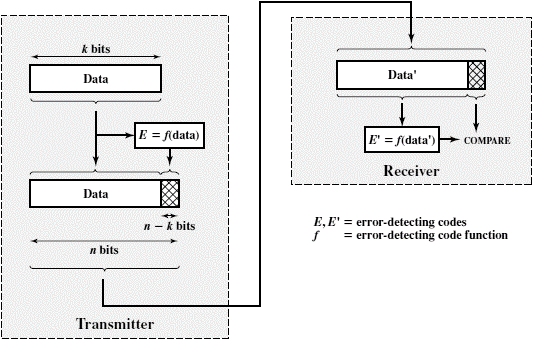
\includegraphics [scale=0.55]{images/Intro/Imagen1.png}
	\caption{Error Detection Process}
\end{figure}



\textbf{Cyclic Redundancy Check (CRC)}\\

One of the most common, and one of the most powerful, error-detecting codes is the
cyclic redundancy check (CRC), which can be described as follows. Given a k-bit
block of bits, or message, the transmitter generates an sequence, known
as a frame check sequence (FCS), such that the resulting frame, consisting of n bits,
is exactly divisible by some predetermined number. The receiver then divides the
incoming frame by that number and, if there is no remainder, assumes there was no
error.3
To clarify this, we present the procedure in three equivalent ways:

\begin{itemize}
	\item Modulo 2 arithmetic
	\item Polynomials
	\item Digital logic
\end{itemize}

The methods seen in class where the first two.\\


\textbf{Modulo 2 arithmetic}\\

Modulo 2 arithmetic uses binary addition with no carries,
which is just the \textbf{ exclusive-OR (XOR)} operation. Binary subtraction with no carries
is also interpreted as the XOR operation.

Now define

\begin{equation*}
	T = 2n-kD + F
\end{equation*}

Where: \\
$P =$ pattern of $n - k + 1$ bits; this is the predetermined divisor\\
$F = (n - k)$-bit FCS, the last $(n - k) $bits of $T$\\
$D =$ $k-$bit block of data, or message, the first $k $bits of $T$\\
$T$= $n$-bit frame to be transmitted \\

According with Tanenbaum \cite \\

CRC (Cyclic Redundancy Check is  also known
as a \textbf{polynomial code}. Polynomial codes are based upon treating bit strings as
representations of polynomials with coefficients of 0 and 1 only. A k-bit frame is
regarded as the coefficient list for a polynomial with $k-$terms, ranging from $x^{k-1}$
to $x^0$.

For example, 110001 has 6 bits and thus represents a six-term polynomial with
coefficients 1, 1, 0, 0, 0, and $ 1: 1x^5 + 1x^4 + 0x^3 + 0x^2 + 0x^1 + 1x^0.$

When the polynomial code method is employed, the sender and receiver must
agree upon a \textbf{ generator polynomial, $\mathbf{G(x)}$}, in advance.  To compute the CRC for some frame with
m bits corresponding to the polynomial $ \mathbf{M(x)}$, the frame must be longer than the
generator polynomial.  When the receiver gets the checksummed frame, it tries dividing it
by G(x). If there is a remainder, there has been a transmission error.

\begin{figure}[!htbp]
	\centering
	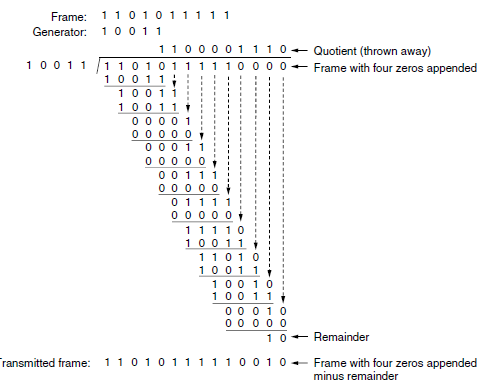
\includegraphics [scale=0.55]{images/Intro/Imagen2.png}
	\caption{Error Detection Process}
\end{figure} 
	\section{Develop}

\subsection{Implementing CRC code in Transmmitter}
\subsection{Implementing CRC code in Receptor}
\subsection{Testing transmission}
\subsection{Frame Error Rate}
\subsection{Friss Equation and Shannon-Hartley Capacity}

	\section{Conclusions}
	
	\phantom{  \cite{stallings2000}}
	\phantom{ \cite{tanenbaumwetherall2014} }
	\phantom{ \cite{teleradio_2020}}
	
	\bibliographystyle{ieeetran}
	\bibliography{References}
	
	
	
	
\end{document}